% !TeX root = ./forallxyyc-solutions.tex

\stepcounter{chapter} % Introducing ML

\chapter{Natural deduction for ML}

\setcounter{ProbPart}{0}

\problempart
Provide proofs for all of the following:
\begin{earg}
\item $\Box (A\eand B)\vdash_\mlK \Box A \eand \Box B$

\myanswer{
\[\begin{nd}
\hypo{1}{\Box (A \eand B)}
\open
\hypo{2}{\ebox}
\have{3}{A \eand B}\boxe{1}
\have{4}{A}\ae{3}
\close
\have{5}{\ebox A}\boxi{3-4}
\open
\hypo{6}{\ebox}
\have{7}{A \eand B}\boxe{1}
\have{8}{B}\ae{7}
\close
\have{9}{\ebox B}\boxi{6-8}
\have{10}{\Box A \eand \Box B}\ai{5,9}
\end{nd}\]
}

\item $\Box A\eand\Box B\vdash_\mlK \Box( A \eand  B)$

\myanswer{
\[\begin{nd}
\hypo{1}{\Box A \eand \Box B}
\have{2}{\Box A}\ae{1}
\have{3}{\Box B}\ae{1}
\open
\hypo{4}{\ebox}
\have{5}{A}\boxe{2}
\have{6}{B}\boxe{3}
\have{7}{A\eand B}\ai{5,6}
\close
\have{8}{\Box (A\eand B)}\boxi{4-7}
\end{nd}\]
}

\item $\Box A\eor\Box B\vdash_\mlK \Box( A \eor  B)$

\myanswer{
\[\begin{nd}
\hypo{1}{\Box A \eor \Box B}
\open
\hypo{2}{\Box A}
\open
\hypo{3}{\ebox}
\have{4}{A}\boxe{2}
\have{5}{A\eor B}\oi{4}
\close
\have{6}{\ebox(A \eor B)}\boxi{3-5}
\close
\open
\hypo{7}{\Box B}
\open
\hypo{8}{\ebox}
\have{9}{B}\boxe{7}
\have{10}{A\eor B}\oi{9}
\close
\have{11}{\Box (A\eor B)}\boxi{8-10}
\close
\have{12}{\Box(A\eor B)}\oe{1,2-6,7-11}
\end{nd}\]
}

\item $\Box (A \eiff B)\vdash_\mlK  \Box A \eiff \Box B$
\myanswer{
\[\begin{nd}
\hypo{1}{\Box(A\eiff B)}
\open
\hypo{2}{\Box A}
\open
\hypo{3}{\ebox}
\have{4}{A\eiff B}\boxe{1}
\have{5}{A}\boxe{2}
\have{6}{B}\be{4,5}
\close
\have{7}{\ebox B}\boxi{3-6}
\close
\open
\hypo{8}{\Box B}
\open
\hypo{9}{\ebox}
\have{10}{A\eiff B}\boxe{1}
\have{11}{B}\boxe{8}
\have{12}{A}\be{10,11}
\close
\have{13}{\ebox A}\boxi{9-12}
\close
\have{14}{\Box A \eiff \Box B}\bi{2-7, 8-13}
\end{nd}\]
}
\end{earg}

\problempart
Provide proofs for the following (without using Modal Conversion!):
\begin{earg}
\item $\enot\Box A\vdash_\mlK  \Diamond \enot A$
\myanswer{
\[\begin{nd}
\hypo{1}{\enot\Box A}
\open
\hypo{2}{\ebox\enot\enot A}
\open
\hypo{3}{\ebox}
\have{4}{\enot\enot A}\boxe{2}
\have{5}{A}\dne{4}
\close
\have{6}{\ebox A}\boxi{3-5}
\have{7}{\ered}\ne{1,6}
\close
\have{8}{\enot\Box\enot\enot A}\ni{2-6}
\have{9}{\Diamond\enot A}\diadf{8}
\end{nd}\]
}

\item $\Diamond\enot A\vdash_\mlK \enot \Box A$
\myanswer{
\[\begin{nd}
\hypo{1}{\Diamond\enot A}
\have{2}{\enot\Box\enot \enot A}\diadf{1}
\open
\hypo{3}{\ebox A}
\open
\hypo{4}{\ebox}
\open
\hypo{5}{\enot A}
\have{6}{A}\boxe{3}
\have{7}{\ered}\ne{5,6}
\close
\have{8}{\enot\enot A}\ni{5-7}
\close
\have{9}{\ebox\enot\enot A}\boxi{4-8}
\have{10}{\ered}\ne{2,9}
\close
\have{11}{\enot\Box A}\ni{3-10}
\end{nd}\]
}

\item $\enot\Diamond A\vdash_\mlK \Box\enot A$

\myanswer{
\[\begin{nd}
\hypo{1}{\enot\Diamond A}
\open
\hypo{2}{\enot\Box\enot A}
\have{3}{\Diamond A}\diadf{2}
\have{4}{\ered}\ne{1,3}
\close
\have{5}{\enot\enot\Box\enot A}\ni{2-4}
\have{6}{\Box \enot A}\dne{5}
\end{nd}\]
}

\item $\Box\enot A\vdash_\mlK \enot\Diamond A$
\myanswer{
\[\begin{nd}
\hypo{1}{\Box\enot A}
\open
\hypo{2}{\Diamond A}
\have{3}{\enot \Box \enot A}\diadf{2}
\have{4}{\bot}\ne{1,3}
\close
\have{5}{\enot\Diamond A}\by{$\enot$I}{2-4}
\end{nd}\]
}
\end{earg}

\problempart
Provide proofs of the following (and now feel free to use Modal Conversion!):
\begin{earg}
\item $\Box(A\eif B), \Diamond A \vdash_\mlK  \Diamond B$
\myanswer{
\[\begin{nd}
\have{1}{\Box(A\eif B)}
\hypo{2}{\Diamond A}
\have{3}{\enot\Box\enot A}\diadf{2}
\open
\hypo{4}{\ebox\enot B}
\open
\hypo{5}{\ebox}
\have{6}{A\eif B}\boxe{1}
\have{7}{\enot B}\boxe{4}
\have{8}{\enot A}\mt{5,6}
\close
\have{9}{\ebox\enot A}\boxi{5-8}
\have{10}{\ered}\ne{3,9}
\close
\have{11}{\enot\Box\enot B}\ni{4-10}
\have{12}{\Diamond B}\diadf{11}
\end{nd}\]
}

\item $\Box A \vdash_\mlK  \enot\Diamond\enot A$
\myanswer{
\[\begin{nd}
\hypo{1}{\Box A}
\open
\hypo{2}{\Diamond\enot A}
\have{3}{\enot\Box A}\mc{2}
\have{4}{\bot}\ne{1,3}
\close
\have{5}{\enot\Diamond\enot A}\ni{2-4}
\end{nd}\]
}

\item $\enot\Diamond\enot A \vdash_\mlK  \Box A$
\myanswer{
\[\begin{nd}
\hypo{1}{\enot\Diamond\enot A}
\have{2}{\Box\enot\enot A}\mc{1}
\open
\hypo{3}{\ebox}
\have{4}{\enot\enot A}\boxe{2}
\have{5}{A}\dne{4}
\close
\have{6}{\Box A}\boxi{3-5}
\end{nd}\]
}
\end{earg}

\problempart
Provide proofs for the following:
\begin{earg}
\item $P\vdash_\mlT \Diamond P$
\myanswer{
\[\begin{nd}
\hypo{1}{P}
\open
\hypo{3}{\Box \enot P}
\have{4}{\enot P}\rt{3}
\have{5}{\ered}\ne{1,4}
\close
\have{6}{\enot\Box\enot P}\ni{3-5}
\have{7}{\Diamond P}\diadf{6}
\end{nd}\]
}

\item $\vdash_\mlT  (A\eand B)\eor(\enot \Box A\eor\enot\Box B)$
\myanswer{
\[\begin{nd}
\open
\hypo{1}{\Box A\eand\Box B}
\have{2}{\Box A}\ae{1}
\have{3}{\Box B}\ae{1}
\have{4}{A}\rt{2}
\have{5}{B}\rt{3}
\have{6}{A\eand B}\ai{4,5}
\have{7}{(A\eand B)\eor (\enot \Box A\eor \enot \Box B)}\oi{6}
\close
\open
\hypo{8}{\enot(\Box A\eand \Box B)}
\have{9}{\enot\Box A \eor \enot\Box B}\dem{8}
\have{10}{(A\eand B)\eor (\enot\Box A \eor \enot\Box B)}\oi{9}
\close
\have{11}{(A\eand B)\eor (\enot\Box A \eor \enot\Box B)}\tnd{1-7,8-10}
\end{nd}\]
}
\end{earg}

\problempart
Provide proofs for the following:
\begin{earg}
\item $\Box(\Box A\eif B), \Box (\Box B\eif C), \Box A \vdash_\mlSfour \Box\Box C$

\myanswer{
\[\begin{nd}
\have{1}{\Box(\Box A \eif B)}
\have{2}{\Box(\Box B\eif C)}
\hypo{3}{\Box A}
\open
\hypo{4}{\ebox}
\have{5}{\Box A}\rfour{3}
\have{6}{\Box(\Box A\eif B)}\rfour{1}
\have{7}{\Box(\Box B\eif C)}\rfour{2}
\open
\hypo{8}{\ebox}
\have{9}{\Box A}\rfour{5}
\have{10}{\ebox(\ebox A \eif B)}\rfour{6}
\open
\hypo{11}{\ebox}
\have{12}{\ebox A}\rfour{9}
\have{13}{\Box A\eif B}\boxe{10}
\have{14}{B}\ce{12,13}
\close
\have{15}{\ebox B}\boxi{11-14}
\have{16}{\ebox B \eif C}\boxe{7}
\have{17}{C}\ce{15,16}
\close
\have{18}{\Box C}\boxi{8-17}
\close
\have{19}{\Box \Box C}\boxi{4-18}
\end{nd}\]
}

\item $\Box A \vdash_\mlSfour  \Box(\Box A \eor B)$
\myanswer{
\[\begin{nd}
\hypo{1}{\Box A}
\open
\hypo{2}{\ebox}
\have{3}{\Box A}\rfour{1}
\have{4}{\Box A \eor B}\oi{4}
\close
\have{5}{\Box(\Box A \eor B)}\boxi{2-4}
\end{nd}\]
}

\item $\Diamond \Diamond A \vdash_\mlSfour  \Diamond A$
\myanswer{
\[\begin{nd}
\hypo{1}{\Diamond\Diamond A}
\open
\hypo{2}{\ebox\enot A}
\have{3}{\enot\ebox\enot\ediamond A}\diadf{1}
\open
\hypo{5}{\ebox}
\have{6}{\Box\enot A}\rfour{2}
\have{7}{\enot\Diamond A}\mc{6}
\close
\have{12}{\ebox\enot\Diamond A}\boxi{5-7}
\have{13}{\ered}\ne{3,12}
\close
\have{14}{\enot\ebox\enot A}\ni{2-13}
\have{15}{\Diamond A}\diadf{14}
\end{nd}\]
}
\end{earg}

\problempart
Provide proofs for the following:
\begin{earg}
\item $\enot\Box\enot A, \Diamond B\vdash_\mlSfive\Box(\Diamond A \eand \Diamond B)$
\myanswer{
\[\begin{nd}
\have{1}{\enot\Box\enot A}
\hypo{2}{\Diamond B}
\have{3}{\enot\ebox\enot B}\diadf{2}
\open
\hypo{4}{\ebox}
\have{5}{\enot\ebox\enot A}\rfive{1}
\have{6}{\Diamond A}\diadf{5}
\have{7}{\enot\ebox\enot B}\rfive{3}
\have{8}{\Diamond B}\diadf{7}
\have{10}{\Diamond A \eand \Diamond B}\ai{6,8}
\close
\have{11}{\Box(\Diamond A \eand \Diamond B)}\boxi{4-10}
\end{nd}\]
}

\item $A\vdash_\mlSfive\Box\ediamond A$
\myanswer{
\[\begin{nd}
\hypo{1}{A}
\open
\hypo{2}{\ebox\enot A}
\have{3}{\enot A}\rt{2}
\have{4}{\ered}\ne{1,3}
\close
\have{5}{\enot\ebox\enot A}
\open
\hypo{6}{\Box}
\have{7}{\enot\ebox\enot A}\rfive{5}
\have{8}{\Diamond A}\diadf{7}
\close
\have{9}{\Box\Diamond A}\boxi{6-8}
\end{nd}\]
}

\item $\ediamond\ediamond A\vdash_\mlSfive\ediamond A$
\myanswer{
\[\begin{nd}
\hypo{1}{\ediamond\ediamond A}
\have{2}{\enot\ebox\enot \ediamond A}\diadf{1}
\open
\hypo{3}{\ebox}
\open
\hypo{4}{\Box\enot A}
\open
\hypo{5}{\ebox}
\open
\hypo{6}{\ediamond A}
\have{7}{\enot\ebox\enot A}\diadf{6}
\have{8}{\ebox\enot A}\rfour{4}
\have{9}{\ered}\ne{7,8}
\close
\have{10}{\enot\ediamond A}\ni{5-9}
\close
\have{11}{\ebox\enot\ediamond A}\boxi{5-10}
\have{12}{\enot\ebox\enot\ediamond A}\rfive{2}
\have{13}{\ered}\ne{11,12}
\close
\have{14}{\enot\ebox\enot A}\ni{4-13}
\have{15}{\ediamond A}\diadf{14}
\close
\have{16}{\ebox\ediamond A}\boxi{3-15}
\have{17}{\ediamond A}\rt{16}
\end{nd}\]
}
\end{earg}

\chapter{Semantics for ML}

We have presented all of the counter-interpretations diagrammatically. If you would prefer to write them out explicitly, then that would be fine too!

\setcounter{ProbPart}{0}

\problempart
Present counter-interpretations to the following:
\begin{earg}
\item $\enot P \vDash_\mlK  \enot\Diamond P$
\myanswer{
\begin{center}
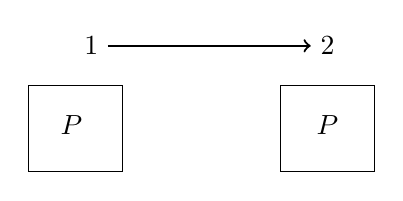
\begin{tikzpicture}
\node (atom1) at (0,1) {1};
\node (atom2) at (3,1) {2};
\node (atom3) at (-0.25,0) {$\enot P$};
\node (atom4) at (3,0) {$P$};
\draw[->, thick] (atom1) -- (atom2);
\draw (-0.8,-0.6) rectangle (0.4,0.5);
\draw (2.4,-0.6) rectangle (3.6,0.5);
\end{tikzpicture}
\end{center}
}

\item $\Box(P \eor Q)\vDash_\mlK  \Box P \eor \Box Q$
\myanswer{
\begin{center}
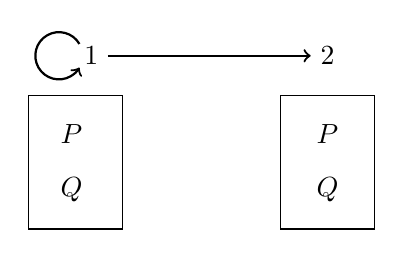
\begin{tikzpicture}
\node (atom1) at (0,1) {1};
\node (atom2) at (3,1) {2};
\node (atom3) at (-0.25,0) {$P$};
\node (atom4) at (3,0) {$\enot P$};
\node (atom5) at (-0.25,-0.7) {$\enot Q$};
\node (atom6) at (3,-0.7) {$Q$};
\draw[->, thick] (atom1)+(-0.15,0.15) arc (-330:-30:.3); 
%\draw[->, thick] (atom2)+(0.15,-0.15) arc (-150:150:.3); 
\draw[->, thick] (atom1) -- (atom2);
\draw (-0.8,-1.2) rectangle (0.4,0.5);
\draw (2.4,-1.2) rectangle (3.6,0.5);
\end{tikzpicture}
\end{center}
}

\item $\vDash_\mlK  \enot \Box (A\eand \enot A)$
\myanswer{
\begin{center}
\begin{tikzpicture}
\node (atom1) at (0,1) {1};
\node (atom3) at (-0,0) {$\enot A$};
\draw (-0.5,-0.6) rectangle (0.6,0.5);
\end{tikzpicture}
\end{center}
}

\item $\Box A\vDash_\mlK  A$
\myanswer{
\begin{center}
\begin{tikzpicture}
\node (atom1) at (0,1) {1};
\node (atom2) at (3,1) {2};
\node (atom3) at (-0.25,0) {$\enot A$};
\node (atom4) at (3,0) {$A$};
\draw[->, thick] (atom1) -- (atom2);
\draw (-0.8,-0.6) rectangle (0.4,0.5);
\draw (2.4,-0.6) rectangle (3.6,0.5);
\end{tikzpicture}
\end{center}
}
\end{earg}

\problempart
Present counter-interpretations to the following:
\begin{earg}
\item $\Box (M\eif O),\Diamond M\vDash_\mlT  O$
\myanswer{
\begin{center}
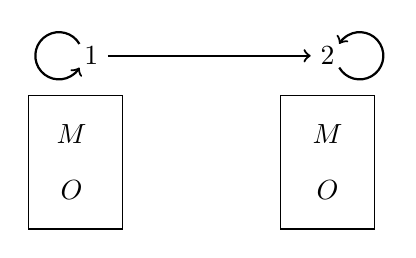
\begin{tikzpicture}
\node (atom1) at (0,1) {1};
\node (atom2) at (3,1) {2};
\node (atom3) at (-0.25,0) {$\enot M$};
\node (atom4) at (3,0) {$M$};
\node (atom5) at (-0.25,-0.7) {$\enot O$};
\node (atom6) at (3,-0.7) {$O$};
\draw[->, thick] (atom1)+(-0.15,0.15) arc (-330:-30:.3); 
%\draw[->, thick] (atom2)+(0.15,-0.15) arc (-150:150:.3); 
\draw[->, thick] (atom1) -- (atom2);
\draw[->, thick] (atom2)+(0.15,-0.15) arc (-150:150:.3); 
\draw (-0.8,-1.2) rectangle (0.4,0.5);
\draw (2.4,-1.2) rectangle (3.6,0.5);
\end{tikzpicture}
\end{center}
}

\item $\Box A\vDash_\mlT  \Box \Box A$
\myanswer{
\begin{center}
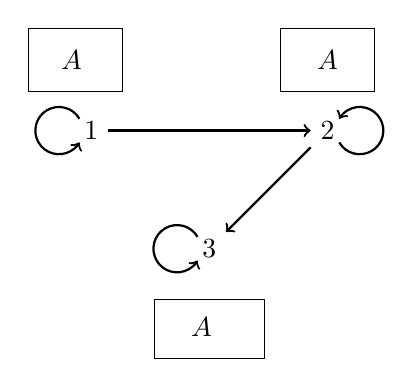
\begin{tikzpicture}
\node (atom1) at (0,1) {1};
\node (atom2) at (3,1) {2};
\node (atom3) at (1.5,-0.5) {3};
\node (atom4) at (-0.25,1.9) {$A$};
\node (atom5) at (3,1.9) {$A$};
\node (atom6) at (1.4,-1.5) {$\enot A$};
\draw[->, thick] (atom1)--(atom2);
\draw[->, thick] (atom1)+(-0.15,0.15) arc (-330:-30:.3); 
\draw[->, thick] (atom2)+(0.15,-0.15) arc (-150:150:.3); 
\draw[->, thick] (atom2)--(atom3);
\draw[->, thick] (atom3)+(-0.15,0.15) arc (-330:-30:.3); 
\draw (-0.8,1.5) rectangle (0.4,2.3);
\draw (2.4,1.5) rectangle (3.6,2.3);
\draw (0.8,-1.15) rectangle (2.2,-1.9);
\end{tikzpicture}
\end{center}
}
\end{earg}

\problempart
Present counter-interpretations to the following:
\begin{earg}
\item $\Diamond A\vDash_\mlSfour  \Box\Diamond A$
\myanswer{
\begin{center}
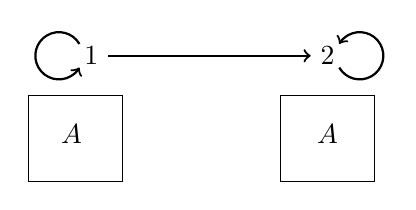
\begin{tikzpicture}
\node (atom1) at (0,1) {1};
\node (atom2) at (3,1) {2};
\node (atom3) at (-0.25,0) {$A$};
\node (atom4) at (3,0) {$\enot A$};
\draw[->, thick] (atom1)+(-0.15,0.15) arc (-330:-30:.3); 
\draw[->, thick] (atom2)+(0.15,-0.15) arc (-150:150:.3); 
\draw[->, thick] (atom1) -- (atom2);
\draw (-0.8,-0.6) rectangle (0.4,0.5);
\draw (2.4,-0.6) rectangle (3.6,0.5);
\end{tikzpicture}
\end{center}
}

\item $\Diamond A, \Box (\Diamond A \eif B)\vDash_\mlSfour \Box B$

\myanswer{
\begin{center}
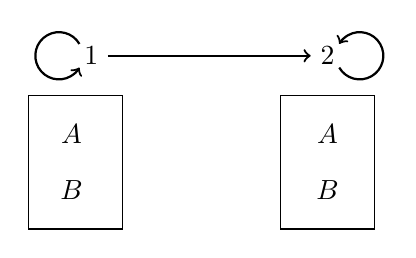
\begin{tikzpicture}
\node (atom1) at (0,1) {1};
\node (atom2) at (3,1) {2};
\node (atom3) at (-0.25,0) {$A$};
\node (atom4) at (3,0) {$\enot A$};
\node (atom5) at (-0.25,-0.7) {$B$};
\node (atom6) at (3,-0.7) {$\enot B$};
\draw[->, thick] (atom1)+(-0.15,0.15) arc (-330:-30:.3); 
\draw[->, thick] (atom2)+(0.15,-0.15) arc (-150:150:.3); 
\draw[->, thick] (atom1) -- (atom2);
\draw (-0.8,-1.2) rectangle (0.4,0.5);
\draw (2.4,-1.2) rectangle (3.6,0.5);
\end{tikzpicture}
\end{center}
}
\end{earg}
